% !TeX program = xelatex
% !TeX encoding = UTF-8
% !TeX root    = documentation.tex
\documentclass{SIBGU-state}

\usepackage{hyperref}
% Метаданные .pdf документа
\hypersetup{pdftitle={Документация для шаблона курсовой}}

\title{Документация к классу документа шаблона курсовой}
\begin{document}

\maketitle
\addtocounter{page}{1}

\tableofcontents

\section*{Введение}
\phantomsection
\addcontentsline{toc}{section}{Введение}

Шаблон курсовой --- класс документа, соответствующий у\-чеб\-но-ме\-то\-ди\-чес\-ко\-му пособию~\cite{bib:recomendations}, разделу 3, компилируемый системой компьютерной вёрстки X\makebox[1.7mm]{\raisebox{-1.1mm}{\reflectbox{E}}}\LaTeX. 

В~классе используются пакеты для~форматирования документа и graphicx для~иллюстраций. Полный список представлен в~приложении~\ref{appendix:used_packages}. В~родительской директории главного .tex файла должен лежать файл чёрно-белого герба для~титульной страницы \verb"MIREA_Gerb_Black" (в~шаблоне используется .eps файл~--- единственный векторный формат, предоставляемый на~сайте вуза~\cite{bib:symbol}, из-за уязвимости .eps файла~\cite{bib:eps_cve} также возможно использование форматов JPEG, PNG).

Документ компилируется в \url{https://overleaf.com} с опцией compiler~--- XeLaTeX. 

Примечание~--- документ скомпилирован \today

\subsection*{Шаблон документа}

Шаблон документа для КР см. в ./additions/document\_template.tex.


\section{Структура документа}

Структура документа совместима со стандартным классом документа extarticle (article). Поддерживаются опции extarticle.


\subsection{Титульная страница}

Рекомендуется использовать выданные преподавателем титульные страницы (например, с~помощью пакета pdfpages).

Пример титульной страницы из~у\-чеб\-но-ме\-то\-ди\-чес\-ко\-го пособия~\cite{bib:recomendations} добавлен в~шаблон ./additions/document\_template.tex.


\subsection{Аннотация}

\begin{verbatim}
	\begin{abstract}
		...
	\end{abstract}
\end{verbatim}

Подраздел аннотации:
\begin{verbatim}
	\subsection*{...}
	...
\end{verbatim}

Пункт аннотации:
\begin{verbatim}
	\subsubsection*{...}
	...
\end{verbatim}

\subsection{Оглавление}

\begin{verbatim}
	\tableofcontents
\end{verbatim}


\subsection{Введение, раздел без нумерации}

\noindent\verb"\section*{"Введение\verb"}"\\
\verb"\phantomsection"\\
\verb"\addcontentsline{toc}{section}{"Введение\verb"}"\\
\verb"..."


\subsection{Раздел}

\begin{verbatim}
	\section{...}
	...
\end{verbatim}

Перед началом раздела в~документ включаются все объявленные, но не~отображённые плавающие окружения.


\subsection{Подраздел}

\begin{verbatim}
	\subsection{...}
	...
\end{verbatim}

Перед началом подраздела в~документ включаются все объявленные, но не~отображённые плавающие окружения.


\subsection{Пункт}

\begin{verbatim}
	\subsubsection{}
	...
\end{verbatim}

Перед началом пункта в~документ включаются все объявленные, но не~отображённые плавающие окружения.


\subsubsection{}

Согласно ГОСТ~\cite{bib:gost732}, пункту 6.2.3, пункты могут иметь только порядковый номер без~заголовка.


\subsection{Список использованных источников}

\begin{verbatim}
	\begin{thebibliography}{99\kern\bibindent}
		\bibitem{...} ...
		...
	\end{thebibliography}
\end{verbatim}

Ссылка на источник:
\begin{verbatim}
	\cite{...}
\end{verbatim}

Пример ссылки на~источник~\cite{bib:recomendations}.

За~наличием ссылок и порядком элементов списка необходимо следить самостоятельно, либо использовать biblatex.


\subsection{Приложение}

Как и в~стандартных классах перед приложениями необходимо указать команду \verb"\appendix".

Пример с~одним приложением:
\begin{verbatim}
	\appendix
	\section{...}
	...
\end{verbatim}

Пример с~тремя приложениями:
\begin{verbatim}
	\appendix
	\section{...}
	...
	\section{...}
	...
	\section{...}
	...
\end{verbatim}

Ссылка на~приложение:
\begin{verbatim}
	\ref{...}
\end{verbatim}

Пример ссылки на~приложение~\ref{appendix:fig_tab_eq_numeration}.

За~порядком приложений необходимо следить самостоятельно.


\subsection{Перечни}


\subsubsection{}

\begin{verbatim}
	\begin{itemize}
		\item ...,
		...
	\end{itemize}
\end{verbatim}

\begin{itemize}
	\item[] Пример простого перечня с~тире:
	\item первый элемент,
	\item второй элемент.
\end{itemize}


\subsubsection{}

\begin{verbatim}
	\begin{enumerate}
		\item ...,
		...
	\end{enumerate} 
\end{verbatim}

\begin{enumerate}
	\item[] Пример простого перечня с~закрывающей скобкой и числом:
	\item первый элемент,
	\item второй элемент.
\end{enumerate}

\begin{enumerate}[label=\asbuk*), ref=\asbuk*]
	\item[] Пример простого перечня с~закрывающей скобкой и буквой:
	\item а;
	\item б;
	\item в;
	\item г;
	\item д;
	\item е;
	\item ж;
	\item и;
	\item к;
	\item л;
	\item м;
	\item н;
	\item о;
	\item п;
	\item р;
	\item с;
	\item т;
	\item у;
	\item ф;
	\item x;
	\item ц;
	\item ш;
	\item э;
	\item ю;
	\item я, при~наличии б\'ольшего количества элементов компилятор выдаст ошибку.
\end{enumerate}


\subsubsection{}

\begin{enumerate}
	\item[] Пример сложного перечня:
	\item первый уровень вложенности,
	\begin{enumerate}
		\item второй уровень вложенности;
		\begin{itemize}
			\item третий уровень вложенности;
			\item элемент;
			\item элемент.
		\end{itemize}
	\end{enumerate}
\end{enumerate}


\subsection{Иллюстрация}

Пакет graphicx подключён.

\begin{verbatim}
	\begin{figure}[htb]
		\centering
		\includegraphics[width=.9\textwidth]{...}
		\parskip=6pt
		\caption{...}
		\label{...}
	\end{figure}
\end{verbatim}

См. рисунок~\ref{fig:test_label} на~с.~\pageref{fig:test_label}, рисунок~\ref{fig:in_appendix} (в~приложении).

\begin{figure}[htb]
	\centering
	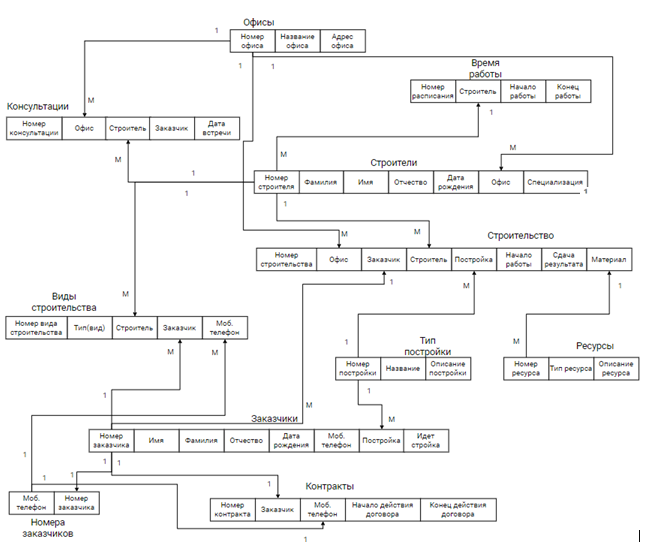
\includegraphics[width=.5\textwidth]{ris/ris3.png}
	\parskip=6pt
	\caption{Подпись ниже рисунка по~центру}
	\label{fig:test_label}
\end{figure}

Обратите внимание, что окружение figure является \emph{плавающим} в~пределах раздела, и иллюстрация может появиться не~там, где Вы ожидаете. Для размещения иллюстрации в~конкретное место необходимо воспользоваться опцией H из~пакета float (не~подключён).


\subsection{Таблица}

См. таблицу~\ref{tab:test_label} на~с.~\pageref{tab:test_label}, таблицу~\ref{tab:in_appendix} (в~приложении).

\begin{verbatim}
	\begin{table}[htb]
		\caption{...}
		\centering
		\begin{tabular}{|c|c|} 
			\hline
			1 & 2 \\ \hline
			3 & 4 \\ \hline
		\end{tabular}
		\label{...}
	\end{table}
\end{verbatim}

\begin{table}[htb]
	\caption{Подпись над таблицей слева без абзацного отступа}
	\centering
	\begin{tabular}{ |c|c|c|c|c| } 
		\hline
		Ячейка 1 & Ячейка 2 & Ячейка 3 & Ячейка 4 & Ячейка 5 \\ \hline
		Ячейка 6 & Ячейка 7 & Ячейка 8 & Ячейка 9 & Ячейка 10 \\ \hline
	\end{tabular}
	\label{tab:test_label}
\end{table}

Обратите внимание, что окружение table является \emph{плавающим} в~пределах раздела, и таблица может появиться не~там, где Вы ожидаете. Для размещения таблицы в~конкретное место необходимо воспользоваться опцией H из~пакета float (не~подключён).


\subsection{Уравнение и формула}

\begin{verbatim}
	\begin{equation}
		a = b ,
	\end{equation}\par
\end{verbatim}\vspace{-.5cm}
{где \verb"$a$~---" первая переменная; \verb"\\" \\
	\verb"$b$~---" вторая переменная.}\bigskip

См. формулу~(\ref{eq:test_label}) в~подразделе, формулу~(\ref{eq:in_appendix}) в~приложении.

\begin{equation}\label{eq:test_label}
	\text{минус}\,a\times b=c ,
\end{equation}

где $a$~--- первая переменная; \\
$b$~--- вторая переменная; \\
$c$~--- третья переменная.

\BeforeBeginEnvironment{thebibliography}{\clearpage\phantomsection}


\begin{thebibliography}{99\kern\bibindent}
	% Пример сервиса для форматирования библиографии https://open-resource.ru/spisok-literatury/
	\bibitem{bib:recomendations} Мерсов, А.А., Русаков, А.М., Филатов, В.В. Методические рекомендации по~выполнению курсовой работы по~дисциплине «Языки программирования».~--- М.: МИРЭА~--- Российский технологический университет, 2022.~--- 73 с.
	\bibitem{bib:symbol} Символика Университета // РТУ МИРЭА Режим доступа: \url{https://www.mirea.ru/mediapage/the-symbolism-of-the-university/}, свободный (дата обращения: 31.05.2022).
	\bibitem{bib:eps_cve} CVE-2013-4979 Detail // CVE Режим доступа: \url{https://www.cve.org/CVERecord?id=CVE-2013-4979}, свободный (дата обращения: 22.06.2022).
	\bibitem{bib:githubrepo} Шаблон XeLaTeX для~курсовой работы по~дисциплине <<Языки программирования>> // GitHub Режим доступа: \url{https://github.com/ValeryVerkhoturov/mirea-kb2-programming-languages}, свободный (дата обращения: 29.05.2022).
	\bibitem{bib:smko} СМКО МИРЭА 7.5.1/03.П.69-16 <<Рекомендации по~оформлению письменных работ обучающихся по~образовательным программам бакалавриата, специалитета, магистратуры>> от~26.10.2016.
	\bibitem{bib:gost732} ГОСТ 7.32-2017. ОТЧЕТ О~НАУЧНО-ИССЛЕДОВАТЕЛЬСКОЙ РАБОТЕ (2017) // Режим доступа: \url{https://docs.cntd.ru/document/1200157208}, свободный.
\end{thebibliography}


\appendix

\section{Используемые пакеты}
\label{appendix:used_packages}

\begin{itemize}
	\item babel,
	\item caption,
	\item enumitem,
	\item fontspec,
	\item geometry,
	\item graphicx,
	\item hyperref,
	\item indentfirst,
	\item newtxmath,
	\item placeins,
	\item titlesec,
	\item tocloft,
	\item ulem.
\end{itemize}

\section{Нумерация иллюстраций и таблиц в~приложении}
\label{appendix:fig_tab_eq_numeration}

\begin{figure}[htb]
	\centering
	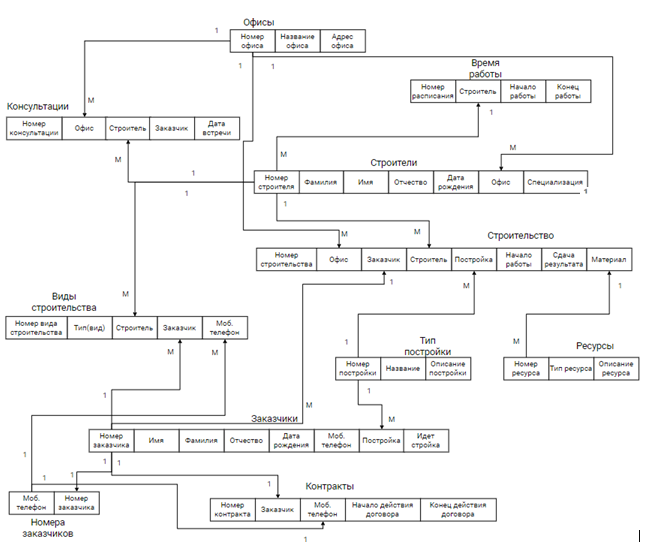
\includegraphics[width=.5\textwidth]{ris/ris3.png}
	\parskip=6pt
	\caption{Иллюстрация в~приложении}
	\label{fig:in_appendix}
\end{figure}

\begin{table}[htb]
	\caption{Таблица в~приложении}
	\centering
	\begin{tabular}{ |c|c|c|c|c| } 
		\hline
		Ячейка 1 & Ячейка 2 & Ячейка 3 & Ячейка 4 & Ячейка 5 \\ \hline
		Ячейка 6 & Ячейка 7 & Ячейка 8 & Ячейка 9 & Ячейка 10 \\ \hline
	\end{tabular}
	\label{tab:in_appendix}
\end{table}

\begin{equation}\label{eq:in_appendix}
	\text{минус}\,a\times b=c ,
\end{equation}

где $a$~--- первая переменная; \\
$b$~--- вторая переменная; \\
$c$~--- третья переменная.


\end{document}